\scanpage{97}
% archive sheet number: 96
\begin{center}
Filtration and weights of the cohomology spaces of algebraic varieties

by A.GROTHENDIECK
\end{center}

0. \uline{Introduction}. It has been observed, since \mbox{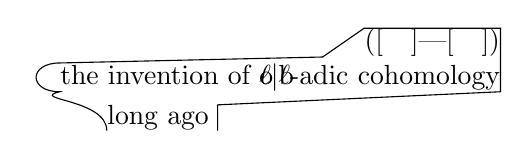
\begin{tikzpicture}[baseline=(old.base)]
\node[inner sep=0] (old) {\deleted{long ago}};
\node[anchor=south west,inner sep=0,xshift=-1.7em,yshift=1.1ex] (added) at (old.north west) {\inserted{the invention of $\unsure{\rlap{o}\handwritten{\ell}|\rlap{b}\handwritten{\ell}}$-ad\handwritten{i\unsure{c}} cohomology}};
\node[anchor=south east,inner sep=0,yshift=.5ex] (ref) at (added.north east) {\handwritten{\unsure{([\quad]|[\quad])}}};
\draw (old.south west) .. controls +(0,.4) and +(-.4,-.1) .. (added.south west) .. controls +(-.4,0) and +(-.4,0) .. (added.north west) -- ([xshift=-1.5em]ref.south west) -- (ref.north west) -- (ref.north east) -- (added.south east) -- ([xshift=.3em]old.north east) .. controls +(0,-.1) and +(0,.2) .. ([xshift=.3em]old.south east);
\end{tikzpicture}}, that\deleted{\unsure{x|,}} for an algebraic variety $X$ defined over a field $k$, with algebraic closure $\bar{k}$, the natural operations of the Galois group $\deleted{\unsure{\operatorname{Gal}k|G_k|G(k)}}\handwritten{\pi}=\operatorname{Gal}(\bar{k}/k)$ on the $\handwritten{\ell}$-adic cohomology $H(X_{\bar{k}},\underline{Z}_{\handwritten{\ell}})$ of the ``geometric'' variety $X_{\bar{k}}$ defined on this \mbox{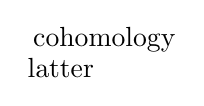
\begin{tikzpicture}[baseline=(old.base)]
\node[inner sep=0] (old) {\deleted{latter}};
\node[anchor=south west,inner sep=0,xshift=.2em,yshift=.4ex] at (old.north west) {\inserted{\handwritten{cohomology}}};
\end{tikzpicture}} a remarkable additional structure, giving rise in particular to the remarkable conjectures of Tate \handwritten{[\quad]}. It seems probable that the latter are n\rlap{\handwritten{o}}\deleted{\unsure{o|e}}t\mbox{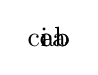
\begin{tikzpicture}[baseline=(old.base)]
\node[inner sep=0] (old) {\deleted{ab}};
\node[anchor=base west,inner sep=0] at (old.base west) {\handwritten{i}};
\node[anchor=base,inner sep=0,xshift=-.3em] at (old.base) {\handwritten{cea}};
\node[anchor=base east,inner sep=0] at (old.base east) {\handwritten{b}};
\end{tikzpicture}}ly further fro\rlap{\handwritten{m}}\deleted{their solution} their solution than the Weil conjectures \handwritten{[\quad,\quad]}, which, as is known, can also be interpreted in terms of Galois actions on $\handwritten{\ell}$-adic cohomology groups. Our purpose in the present work is to show how one can, from the Weil conjectures and (where applicable) from the resolution of singularities, draw consequences of an apparently ``geometric'' nature, i.e. relative to an algebraically closed base field. The principle \mbox{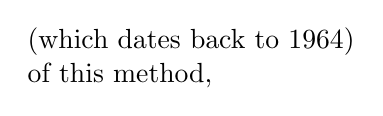
\begin{tikzpicture}[baseline=(base.base)]
\node[inner sep=0] (base) {of this method,};
\node[anchor=south west,inner sep=0,yshift=.6ex] at (base.north west) {\inserted{\deleted{(which dates back to 1964)}}};
\end{tikzpicture}} which thus consists essentially in reducing a geometric statement to the case of a finite base field, is explained in number\textsuperscript{\uline{}} 1, and examples of the application of this method are given in numbers 2 to 7. \deleted{The pr} The idea of these arguments, linked to \mbox{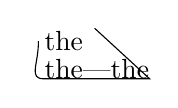
\begin{tikzpicture}[baseline=(old.base)]
\node[inner sep=0] (old) {\deleted{\unsure{the|the}}};
\node[anchor=south west,inner sep=0,yshift=.6ex] (added) at (old.north west) {\inserted{the}};
\draw ([xshift=-.2em]added.west) .. controls +(0,-.3) and +(-.2,0) .. (old.south west) -- (old.south east) -- ([xshift=.4em,yshift=.1em]added.north east);
\end{tikzpicture}} \mbox{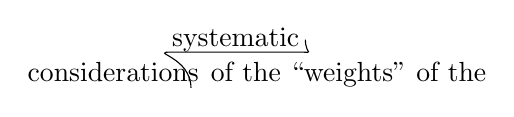
\begin{tikzpicture}[baseline=(base.base)]
\node[inner sep=0] (base) {consideration\deleted{\unsure{s}}};
\node[anchor=base west,inner sep=0,xshift=.4em] (right) at (base.base east) {of the ``weights'' of the};
\node[anchor=south west,inner sep=0,xshift=-1em,yshift=.8ex] (added) at (base.north east) {\inserted{systematic}};
\draw ([xshift=-.3em,yshift=-.5ex]base.south east) .. controls +(0,.4) and +(-.3,0) .. (added.south west) -- (added.south east) .. controls +(.2,0) and +(0,-.2) .. ([xshift=.2em]added.east);
\end{tikzpicture}} Galois modules coming from $\handwritten{\ell}$-adic cohomology, dates back to 1964; \mbox{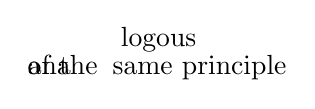
\begin{tikzpicture}[baseline=(du.base)]
\node[inner sep=0] (du) {\deleted{of the}};
\node[anchor=base west,inner sep=0,xshift=.5em] (old) at (du.base east) {\deleted{same principle}};
\node[anchor=base west,inner sep=0] at (du.base west) {\handwritten{ana}};
\node[anchor=south west,inner sep=0,xshift=.3em,yshift=.2ex] at (old.north west) {\inserted{\handwritten{logous}}};
\end{tikzpicture}} examples are to be found developed in SGA 7\handwritten{(}I and II\handwritten{)}; in the oral seminar\deleted{e} \mbox{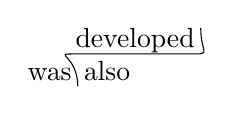
\begin{tikzpicture}[baseline=(left.base)]
\node[inner sep=0] (left) {was};
\node[anchor=base west,inner sep=0,xshift=.4em] (base) at (left.base east) {also};
\node[anchor=south west,inner sep=0,xshift=-.3em,yshift=.6ex] (added) at (base.north west) {\inserted{\handwritten{developed}}};
\draw ([xshift=.2em,yshift=-.4ex]left.south east) .. controls +(0,.4) and +(-.3,0) .. (added.south west) -- (added.south east) .. controls +(.2,0) and +(0,-.3) .. ([xshift=.2em]added.north east);
\end{tikzpicture}} the examp\unsure{\rlap{o}l|\rlap{b}l}e of number\textsuperscript{\uline{}} 2 of the present work.

Of course, the scope of the ``results'' of our work is necessarily \mbox{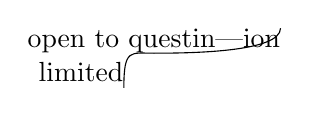
\begin{tikzpicture}[baseline=(old.base)]
\node[inner sep=0] (old) {\deleted{limited}};
\node[anchor=south west,inner sep=0,xshift=-.4em,yshift=.7ex] (added) at (old.north west) {\inserted{\handwritten{open to quest\unsure{in|ion}}}};
\draw ([yshift=-.5ex]old.south east) .. controls +(0,.5) and +(-.3,0) .. (added.south) .. controls +(.5,0) and +(0,-.3) .. (added.north east);
\end{tikzpicture}}, since they depend on conjectures unproved at the present time, namely the Weil conjectures and the resolution of singularities (in Hironaka's strong form) in characteristic
